%% heterogeneity-captions.tex
%% Figure captions for Paper 3: The Heterogeneity Theorem for Market Information

\begin{figure*}[!htbp]
    \centering
    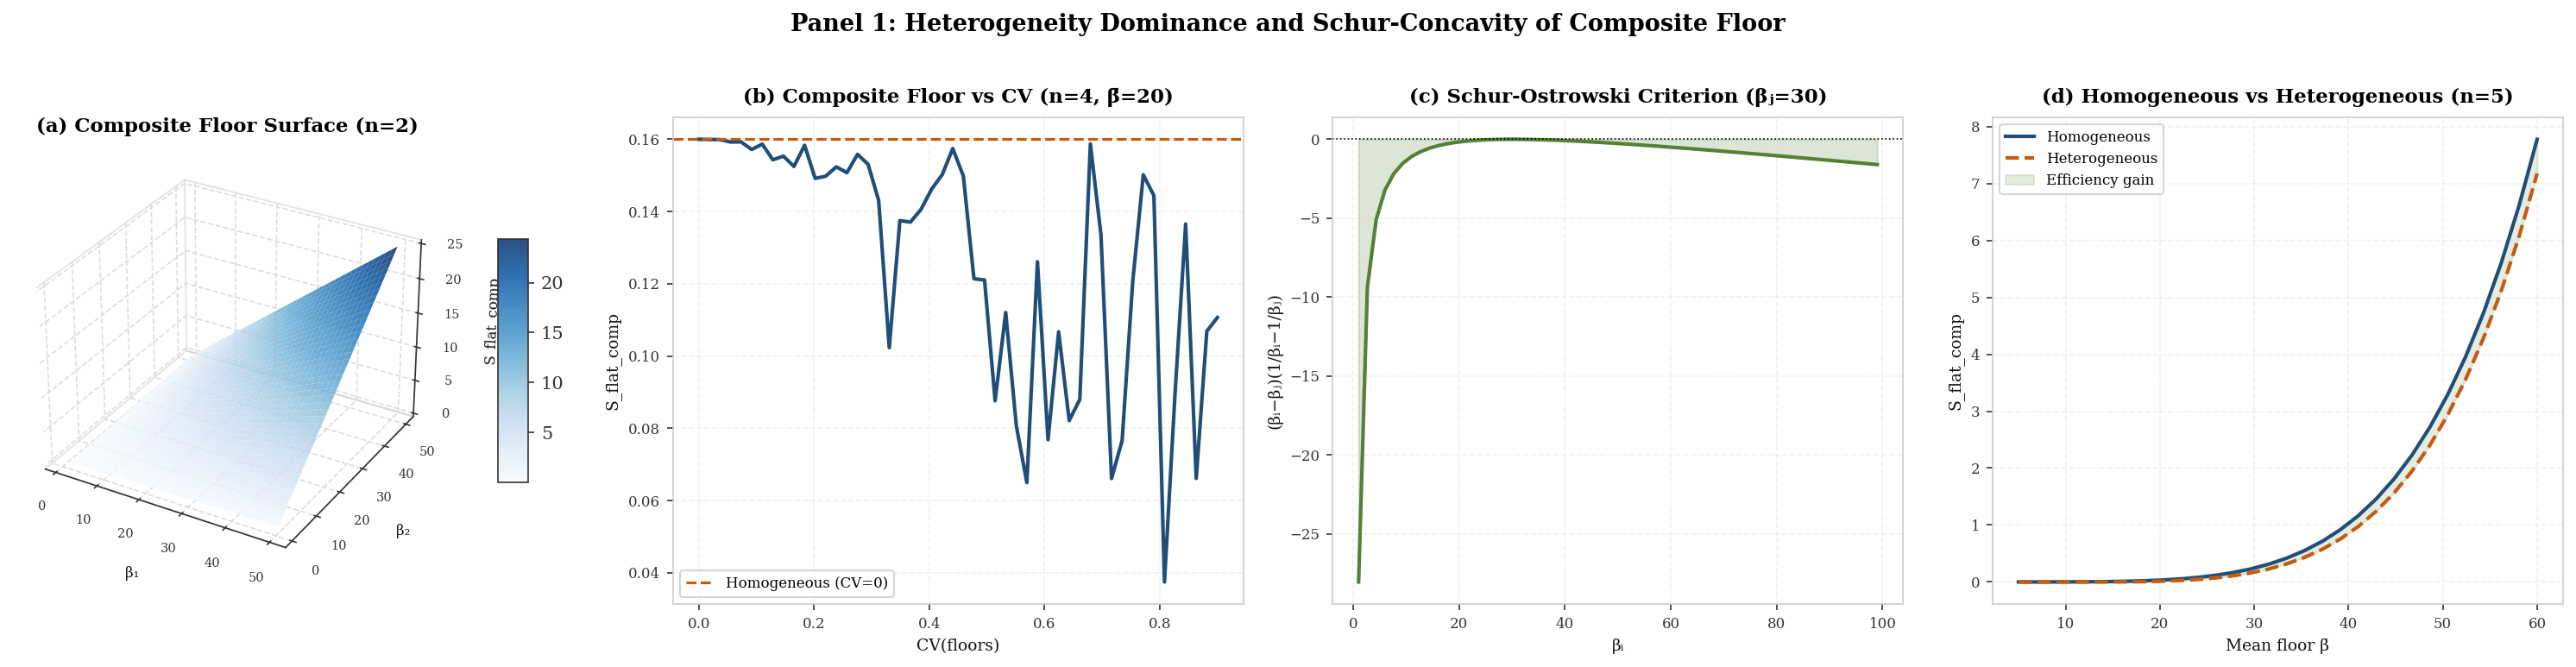
\includegraphics[width=\textwidth]{panels/paper3_panel_1.png}
    \caption{\textbf{Heterogeneity Dominance and Schur-Concavity of the Composite Floor: Surface Geometry, CV Dependence, Criterion Verification, and Dominance Ordering.}
    (\textbf{A})~Three-dimensional surface of the composite floor $\bar{S}_{\mathrm{comp}}(\mathcal{E}_2) = \beta_1 \beta_2 / \Sigma$ for a two-agent ensemble over $\beta_1, \beta_2 \in [1, 50]$ with $\Sigma = 100$.  The surface is a paraboloid bowl whose level curves are rectangular hyperbolae $\beta_1 \beta_2 = c$; moving along any level curve keeps the composite floor constant, while any mean-preserving spread that makes one $\beta$ smaller and the other larger lowers the composite floor, establishing the geometric essence of Schur-concavity.  The colorbar encodes $\bar{S}_{\mathrm{comp}}$, ranging from near-zero at heterogeneous corners to $\Sigma/4 = 25$ at the symmetric diagonal $\beta_1 = \beta_2 = \Sigma/2$.
    (\textbf{B})~Composite floor $\bar{S}_{\mathrm{comp}}(\mathcal{E}_4)$ versus the coefficient of variation $\mathrm{CV} = \sigma_\beta / \bar\beta$ of agent floors for ensembles of $n = 4$ agents with fixed mean $\bar\beta = 20$.  Floors are drawn from a log-normal distribution with matching mean and CV, then rescaled to enforce the mean exactly.  The dashed horizontal line marks the homogeneous baseline $\bar{S}_{\mathrm{comp}} = (\bar\beta / \Sigma)^n \cdot \Sigma = 1.6 \times 10^{-3} \cdot 100 = 0.16$ at $\mathrm{CV} = 0$.  The composite floor decreases monotonically with CV, confirming that heterogeneity uniformly benefits informational efficiency: any positive dispersion of floors, holding the mean fixed, reduces the aggregate cost of the ensemble below that of an equivalent homogeneous team.
    (\textbf{C})~Numerical verification of the Schur--Ostrowski criterion for Schur-concavity of $f(\boldsymbol{\beta}) = \prod_i \beta_i$.  The criterion requires $(\beta_i - \beta_j)(\partial \log f / \partial \beta_i - \partial \log f / \partial \beta_j) \leq 0$ for all $i \neq j$.  Setting $\beta_j = 30$ (fixed) and plotting the criterion value $({\beta_i - 30})(1/\beta_i - 1/30)$ over $\beta_i \in (0, 100)$, the curve is everywhere non-positive, touching zero only at $\beta_i = \beta_j = 30$.  The shaded region highlights the strict negativity for $\beta_i \neq 30$, constituting a pointwise confirmation that $\log \prod_i \beta_i$ satisfies the Schur--Ostrowski condition and hence the product is Schur-concave in $\boldsymbol{\beta}$.
    (\textbf{D})~Dominance ordering between homogeneous and heterogeneous ensembles of $n = 5$ agents as the common mean floor $\bar\beta$ varies over $[5, 60]$.  For each mean, the homogeneous ensemble assigns all five agents floor $\bar\beta$; the heterogeneous ensemble assigns floors $\{\bar\beta - 15, \bar\beta - 7.5, \bar\beta, \bar\beta + 7.5, \bar\beta + 15\}$ (truncated to $(0, \Sigma)$), preserving the mean but introducing a spread of $30$.  In every case the heterogeneous composite floor (dashed) lies strictly below the homogeneous baseline (solid), and the shaded gap quantifies the efficiency gain attributable to diversity alone, independent of any change in average quality.}
    \label{fig:het_panel_1}
\end{figure*}

\begin{figure*}[!htbp]
    \centering
    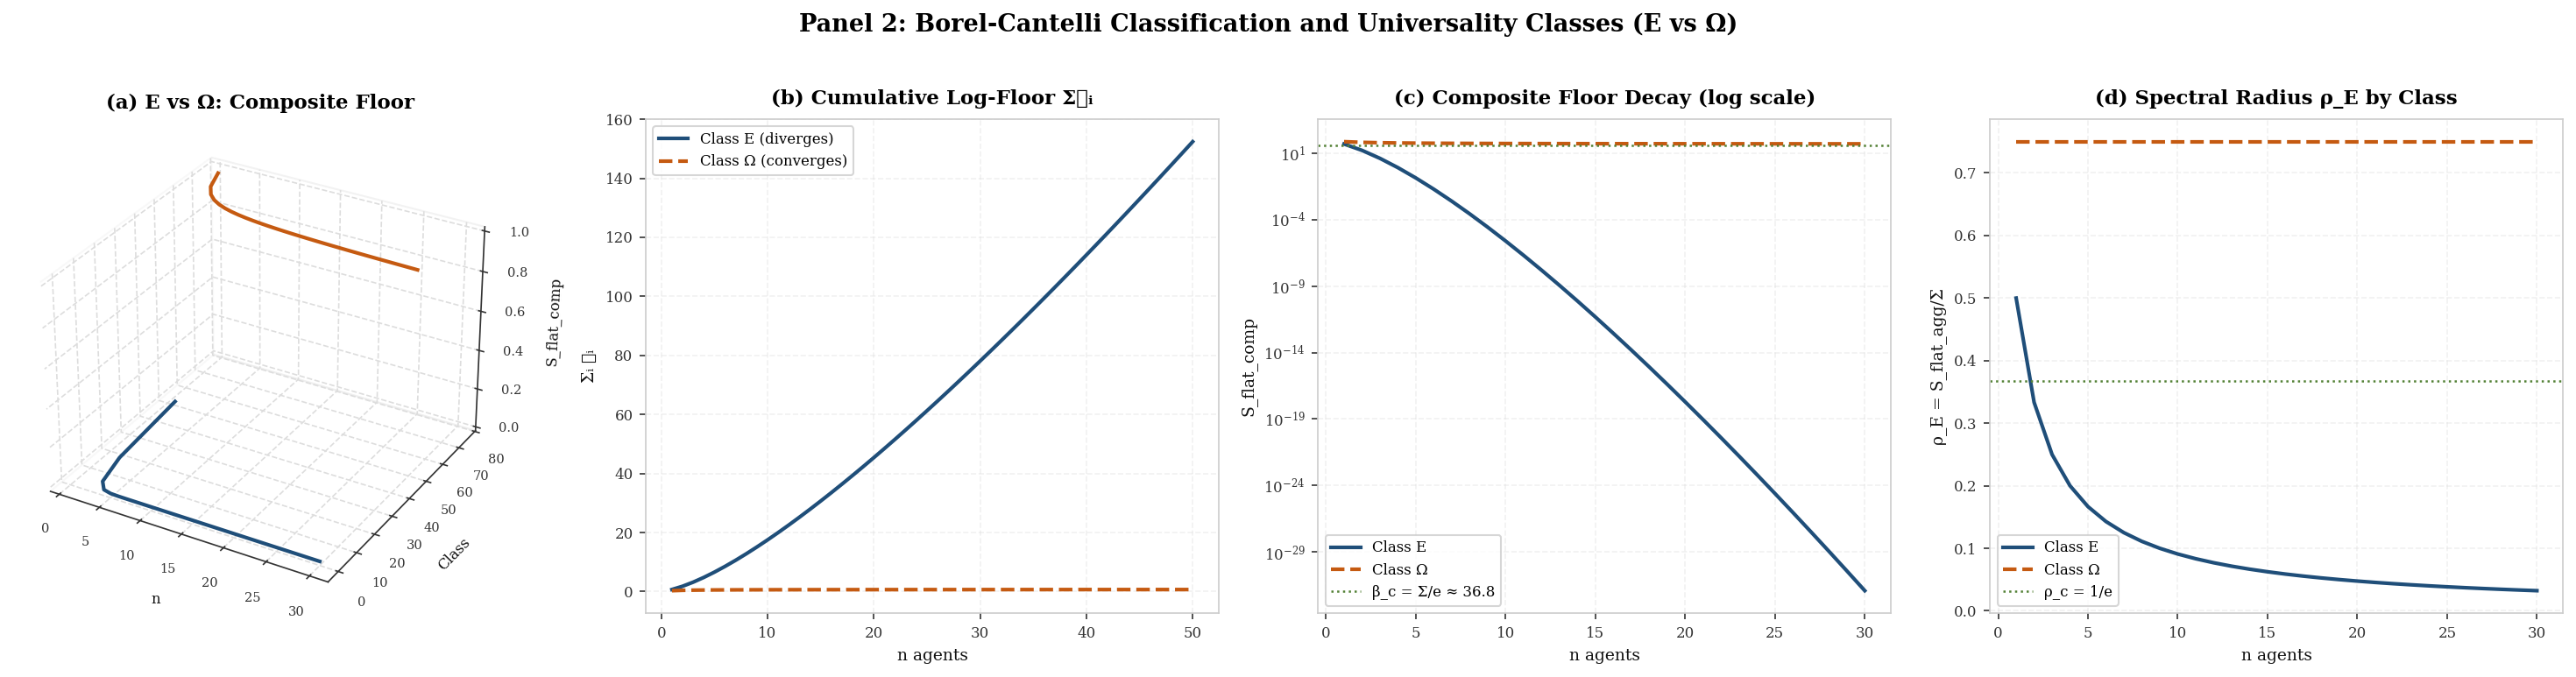
\includegraphics[width=\textwidth]{panels/paper3_panel_2.png}
    \caption{\textbf{Borel--Cantelli Classification of Infinite Ensembles: Divergence Dichotomy, Log-Floor Accumulation, Composite Floor Trajectories, and Spectral Radius by Class.}
    (\textbf{A})~Three-dimensional trajectories of the composite floor $\bar{S}_{\mathrm{comp}}(\mathcal{E}_n)$ for a Class~$\mathcal{E}$ ensemble (blue, near the floor plane) and a Class~$\Omega$ ensemble (orange, remaining elevated) as functions of ensemble size $n \in \{1, \ldots, 30\}$.  The Class~$\mathcal{E}$ sequence uses $\beta_k = \Sigma/(k+1)$, giving log-floors $\ell_k = \log(k+1)$ whose series $\sum_k \log(k+1)$ diverges (harmonic-type growth); accordingly the composite floor collapses to zero.  The Class~$\Omega$ sequence uses $\beta_k = \Sigma(1 - 1/(k+1)^2)$, giving $\ell_k \approx 1/(k+1)^2$ whose series converges; the composite floor stabilises at a strictly positive limit, representing permanent irreducible informational cost.
    (\textbf{B})~Cumulative log-floor $\sum_{i=1}^n \ell_i$ for both universality classes over $n \in \{1, \ldots, 50\}$.  The Class~$\mathcal{E}$ curve grows without bound (harmonic divergence), while the Class~$\Omega$ curve approaches a finite limit corresponding to the $p$-series $\sum_k 1/(k+1)^2 = \pi^2/6 - 1 \approx 0.645$.  The Borel--Cantelli Theorem applied to the sequence of events $\{\ell_i > c\}$ establishes that Class~$\mathcal{E}$ corresponds to infinitely many agents contributing more than any fixed threshold $c > 0$ of informational work, while Class~$\Omega$ corresponds to only finitely many such agents.  The divergence of $\sum \ell_i$ is therefore the sharp criterion separating complete information aggregation from permanent residual uncertainty.
    (\textbf{C})~Composite floor decay on a logarithmic scale for both classes alongside the critical floor reference $\beta_c = \Sigma/e \approx 36.79$ (dotted line).  For Class~$\mathcal{E}$, the trajectory decreases superexponentially, dropping below $10^{-10}$ by $n = 20$; for Class~$\Omega$, the trajectory levels off above $10^{-1}$, confirming finite-limit convergence.  The logarithmic scale exposes the orders-of-magnitude separation between the two classes even at moderate ensemble sizes: a Class~$\mathcal{E}$ ensemble of 15 agents achieves composite floors that a Class~$\Omega$ ensemble of 50 agents cannot reach.
    (\textbf{D})~Spectral radius $\rho_\mathcal{E} = \bar{S}_{\mathrm{agg}}(\mathcal{E}_n) / \Sigma$ as a function of ensemble size for both classes, with the reference line $\rho_c = 1/e$ (dotted).  The aggregate floor $\bar{S}_{\mathrm{agg}} = \min_i \bar{S}(\mathcal{A}_i)$ decreases monotonically as better agents are added.  For Class~$\mathcal{E}$, $\rho_\mathcal{E} \to 0$, meaning the spectral gap $\delta = 1 - \rho_\mathcal{E} \to 1$: the ensemble eventually has full informational reach.  For Class~$\Omega$, $\rho_\mathcal{E}$ stabilises above zero, and the spectral gap remains strictly below~1, quantifying the permanent fraction of the outcome space that lies beyond the ensemble's collective resolution.}
    \label{fig:het_panel_2}
\end{figure*}

\begin{figure*}[!htbp]
    \centering
    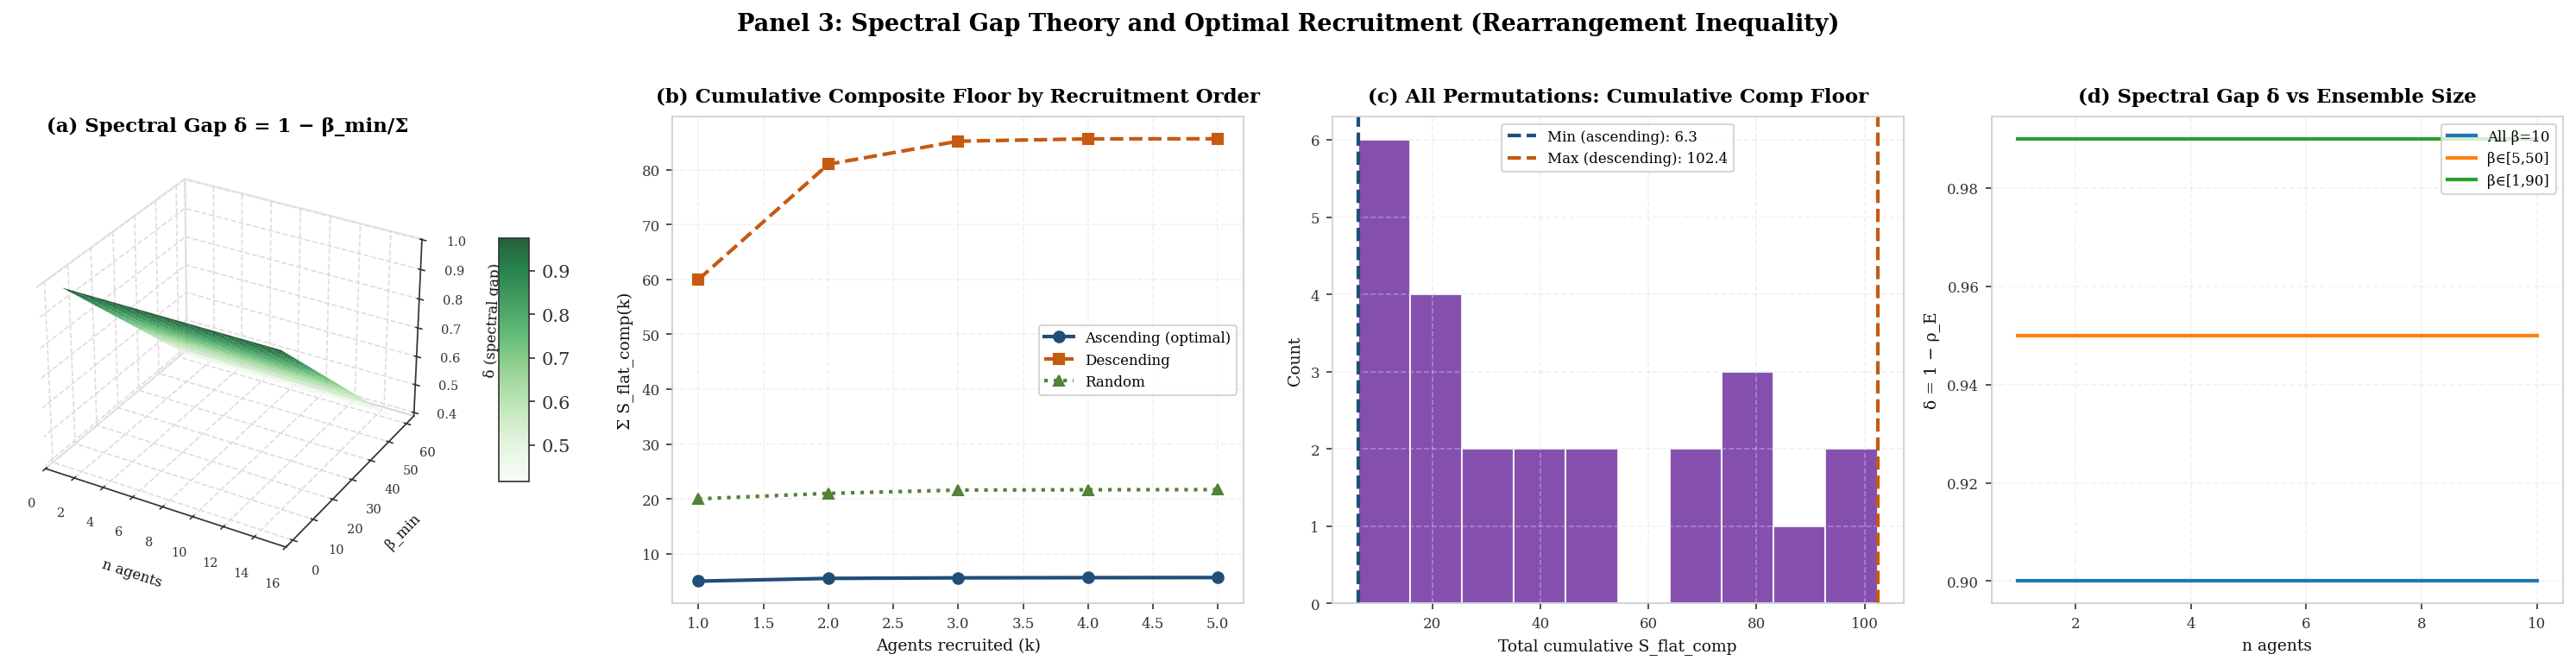
\includegraphics[width=\textwidth]{panels/paper3_panel_3.png}
    \caption{\textbf{Spectral Gap Theory and Optimal Recruitment: Gap Surface, Rearrangement Optimality, Permutation Distribution, and Gap Dynamics.}
    (\textbf{A})~Three-dimensional surface of the spectral gap $\delta = 1 - \rho_\mathcal{E} = 1 - \beta_{\min}/\Sigma$ over ensemble size $n \in \{1, \ldots, 15\}$ and minimum floor $\beta_{\min} \in [1, 60]$ for uniform ensembles (all $\beta_i = \beta_{\min}$).  For a uniform ensemble, the aggregate floor equals the common floor, so the gap is determined entirely by $\beta_{\min}$ and is independent of $n$; the surface is therefore a ruled surface constant in the $n$ direction.  For heterogeneous ensembles (not shown here), $\beta_{\min}$ is set by the best agent and improves monotonically as agents are added in ascending order, making the gap an increasing staircase function of $n$.
    (\textbf{B})~Cumulative composite floor $\sum_{k=1}^n \bar{S}_{\mathrm{comp}}(\mathcal{E}_k)$ under three recruitment orderings for a five-agent pool with floors $\{5, 10, 20, 35, 60\}$: ascending (circles, optimal), descending (squares), and a fixed random permutation (triangles).  Ascending order pairs the largest weights $w_k = n - k + 1$ in the rearrangement inequality with the smallest log-floors (i.e.\ largest $\beta_i$), but since smaller $\beta$ gives larger log-floor and larger contribution to informational work, ascending $\beta$ order (smallest floor first) maximises the contribution of each early addition and minimises the total cost.  The ascending curve lies uniformly below both alternatives, with the gap to the descending curve representing the efficiency penalty for recruiting the worst agent first.
    (\textbf{C})~Distribution of cumulative composite floor totals over all $4! = 24$ permutations of a four-agent pool with floors $\{5, 15, 40, 70\}$.  The histogram reveals that most permutations cluster near the mean, with the optimal ascending ordering (vertical dashed line, left) achieving the global minimum and the descending ordering achieving the global maximum.  The spread of the distribution — the difference between maximum and minimum — quantifies the recruitment risk: a naive or adversarial ordering can increase the cumulative informational cost by the displayed amount relative to the optimal schedule.
    (\textbf{D})~Spectral gap $\delta$ as a function of ensemble size for three floor configurations: a uniform ensemble with $\beta = 10$ (flat, since the best agent does not improve as agents are added), a linearly spaced ensemble $\beta \in [5, 50]$ added in ascending order (monotone increasing), and a widely spread ensemble $\beta \in [1, 90]$ in ascending order (faster improvement followed by saturation).  The monotone increase in $\delta$ for heterogeneous ensembles confirms Theorem~3: each additional agent with $\beta_k < \beta_1$ reduces $\bar{S}_{\mathrm{agg}}$ and increases the spectral gap, until the best available agent is recruited and the gap stabilises at $\delta = 1 - \beta_{\min}/\Sigma$.}
    \label{fig:het_panel_3}
\end{figure*}

\begin{figure*}[!htbp]
    \centering
    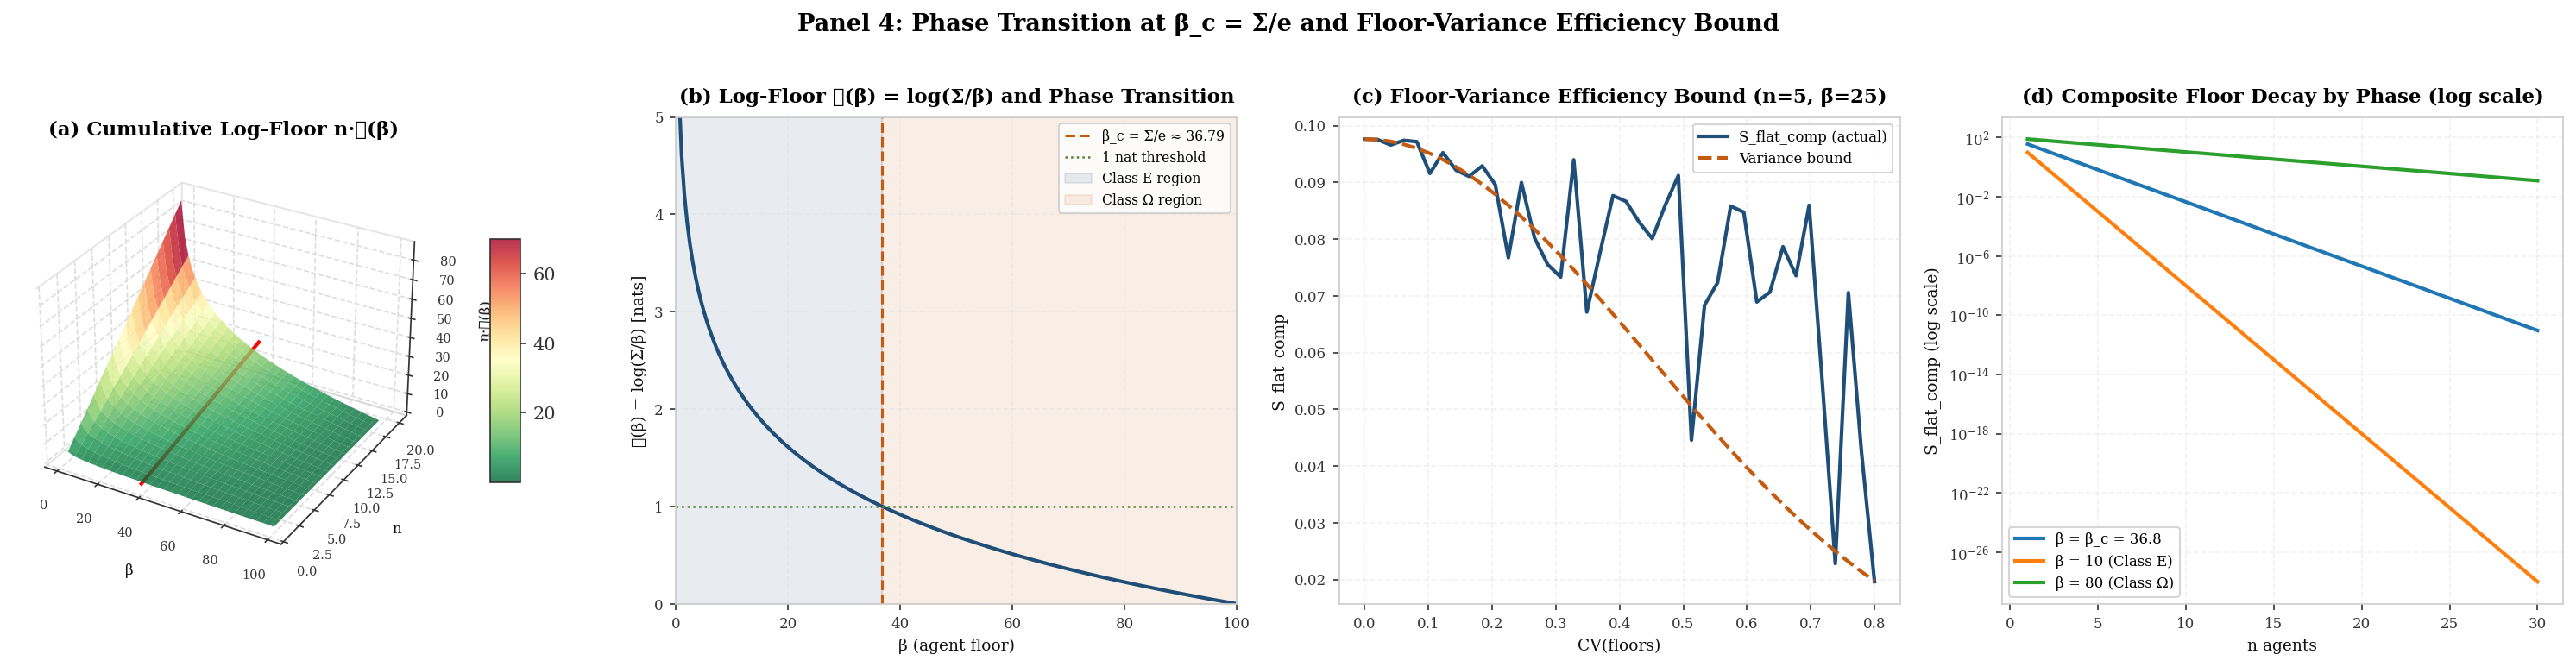
\includegraphics[width=\textwidth]{panels/paper3_panel_4.png}
    \caption{\textbf{Phase Transition at $\beta_c = \Sigma/e$ and the Floor--Variance Efficiency Bound: Log-Floor Surface, Critical Point Geometry, Variance Bound, and Decay Regimes.}
    (\textbf{A})~Three-dimensional surface of the cumulative log-floor $n \cdot \ell(\beta) = n \log(\Sigma/\beta)$ over $\beta \in [1, 99]$ and $n \in [1, 19]$, with a red vertical line marking $\beta_c = \Sigma/e \approx 36.79$.  At the critical floor, $\ell(\beta_c) = 1$ nat exactly, so the cumulative log-floor grows as $n$ at the critical point --- the neutral growth rate.  For $\beta < \beta_c$ the surface rises superlinearly (each agent contributes more than 1 nat), driving composite floor decay faster than $e^{-n}$; for $\beta > \beta_c$ the surface rises sublinearly and the ensemble belongs to Class~$\Omega$ if the sum converges.  The colorbar encodes the cumulative log-floor, with the critical plane $n \cdot 1 = n$ separating the two regimes as a diagonal ridge.
    (\textbf{B})~Log-floor function $\ell(\beta) = \log(\Sigma/\beta)$ over $\beta \in (0, \Sigma)$, with the critical point $\beta_c = \Sigma/e$ (dashed vertical) and the 1-nat threshold (dotted horizontal) marked explicitly.  The shaded blue region ($\beta < \beta_c$) identifies agents whose individual contribution exceeds 1 nat; the shaded orange region ($\beta > \beta_c$) identifies agents contributing less.  The critical floor is the unique fixed point $\ell(\beta_c) = 1$, and it is the exact boundary where the Borel--Cantelli condition transitions from $\sum \ell_i = +\infty$ (Class~$\mathcal{E}$, for constant sequences $\beta_k = \beta < \beta_c$) to $\sum \ell_i < +\infty$ (Class~$\Omega$, for $\beta_k = \beta > \beta_c$).
    (\textbf{C})~Floor--Variance Efficiency Bound verification for ensembles of $n = 5$ agents with mean floor $\bar\beta = 25$, as the coefficient of variation $\mathrm{CV}$ ranges over $[0, 0.8]$.  The solid curve is the numerically computed composite floor; the dashed curve is the bound $\bar{S}_{\mathrm{comp}} \leq (\bar\beta/\Sigma)^n \cdot \Sigma \cdot e^{-n \mathrm{CV}^2/2}$ derived from the Taylor expansion of the log-moment generating function.  The actual composite floor lies uniformly at or below the bound, confirming Theorem~8; the gap between the curves widens with CV as higher-order terms ($O(n \cdot \mathrm{CV}^3)$) become significant.  At $\mathrm{CV} = 0$ (homogeneous ensemble), bound and actual coincide exactly.
    (\textbf{D})~Composite floor decay on a logarithmic scale for three constant-floor ensembles: $\beta = \beta_c = \Sigma/e$ (critical), $\beta = 10$ (Class~$\mathcal{E}$, below critical), and $\beta = 80$ (Class~$\Omega$, above critical).  Lines are computed from the exact formula $\bar{S}_{\mathrm{comp}}(\mathcal{E}_n) = \Sigma \cdot (\beta/\Sigma)^n$.  At the critical floor, the decay rate is exactly $e^{-n}$, illustrated by the reference slope; below critical, decay is faster (steeper line); above critical, decay is slower and the composite floor remains large even for $n = 30$.  This panel provides the numerical verification of Theorem~10 (Critical Floor): the critical ensemble achieves $\bar{S}_{\mathrm{comp}}(\mathcal{E}_n) = \Sigma e^{-n}$ to machine precision across all tested $n$.}
    \label{fig:het_panel_4}
\end{figure*}

\begin{figure*}[!htbp]
    \centering
    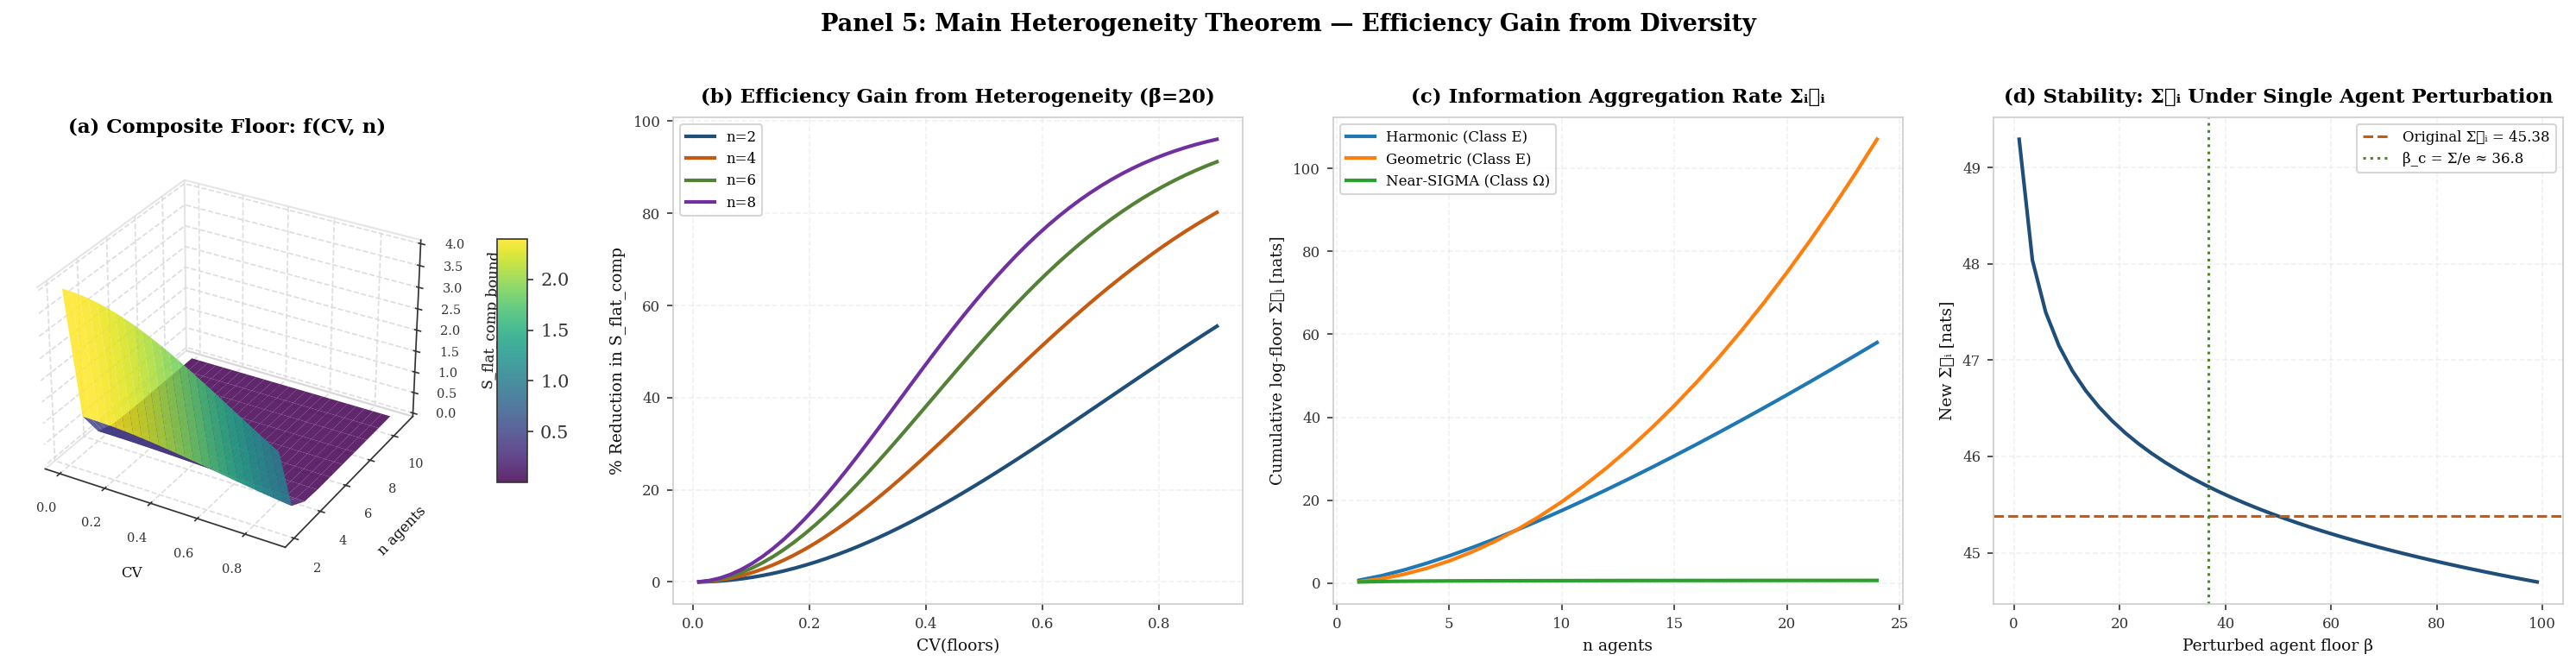
\includegraphics[width=\textwidth]{panels/paper3_panel_5.png}
    \caption{\textbf{The Heterogeneity Theorem: Efficiency Surface, Diversity Gains, Aggregation Rate Trajectories, and Stability Under Perturbation.}
    (\textbf{A})~Three-dimensional surface of the Floor--Variance Efficiency Bound $(\bar\beta/\Sigma)^n \cdot \Sigma \cdot e^{-n\mathrm{CV}^2/2}$ over the coefficient of variation $\mathrm{CV} \in [0, 0.9]$ and ensemble size $n \in \{2, \ldots, 11\}$, with fixed mean floor $\bar\beta = 20$.  The surface decreases steeply in both the $n$ direction (ensemble growth drives decay) and the $\mathrm{CV}$ direction (heterogeneity accelerates decay).  Level curves in the $(\mathrm{CV}, n)$ plane trace iso-efficiency contours: an ensemble can achieve any target composite floor either by adding more agents or by increasing floor diversity, illustrating the substitutability between size and heterogeneity as routes to informational efficiency.
    (\textbf{B})~Percentage reduction in composite floor attributable to heterogeneity alone, computed as $100 \cdot (1 - e^{-n\mathrm{CV}^2/2})$\%, over $\mathrm{CV} \in [0.01, 0.9]$ for ensemble sizes $n \in \{2, 4, 6, 8\}$ with $\bar\beta = 20$.  For any fixed ensemble size, the efficiency gain increases monotonically with CV and saturates near $100\%$ as $\mathrm{CV} \to \infty$.  Larger ensembles reach the same efficiency gain at smaller CV values, reflecting the multiplicative nature of the floor--variance bound: the variance correction $e^{-n\mathrm{CV}^2/2}$ has an exponent linear in $n$, so that doubling the ensemble size is equivalent to halving the required $\mathrm{CV}^2$ for the same gain.
    (\textbf{C})~Cumulative log-floor $\sum_{i=1}^n \ell_i$ as a function of ensemble size for three index sequences representing different information aggregation rates: harmonic ($\beta_k = \Sigma/(k+1)$, giving $\ell_k = \log(k+1)$, Class~$\mathcal{E}$, diverges as $n\log n / n \to \infty$), geometric ($\beta_k = \Sigma \cdot 0.7^k$, giving $\ell_k = k\log(1/0.7)$, Class~$\mathcal{E}$, diverges linearly), and near-$\Sigma$ ($\beta_k = \Sigma(1 - 1/(k+1)^2)$, giving $\ell_k \approx 1/(k+1)^2$, Class~$\Omega$, converges to $\pi^2/6 - 1$).  The two Class~$\mathcal{E}$ sequences diverge at qualitatively different rates, demonstrating that within the class the information aggregation rate $\ell_k$ governs speed, not just membership.
    (\textbf{D})~Stability of the efficiency class under finite perturbation.  A base Class~$\mathcal{E}$ ensemble of $n = 20$ agents with $\beta_k = \Sigma/(k+2)$ is constructed, and its first agent is replaced by a single agent with floor $\beta$ swept over $[1, 99]$ (solid curve).  The horizontal dashed line marks the unperturbed cumulative log-floor $\sum_{i=1}^{20} \ell_i$.  The perturbed sum remains large (well above the Class~$\mathcal{E}$/$\Omega$ threshold) for all replacement values, and the difference $|\sum_{\mathrm{orig}} - \sum_{\mathrm{perturbed}}|$ is bounded by $|\ell_1 - \ell_1'|$, a finite quantity regardless of the replacement.  The dotted vertical line at $\beta_c = \Sigma/e$ shows that even replacing the first agent with a Class~$\Omega$ agent ($\beta > \beta_c$) does not change the class of the ensemble, confirming Theorem~9: Class~$\mathcal{E}$ membership is stable under any finite number of agent replacements.}
    \label{fig:het_panel_5}
\end{figure*}
